\section*{Coding Scheme}
\begin{table}
\begin{tabular}{|c|l|}
\hline 
On the tablet & Releasing the widget\\
& Searching with the widget\\
& Retrying the level\\
& Ending the level before the time is up\\
& Fidgeting with the widget in their hands\\
\hline 
Facial expression & Frowning, annoyance, aggression\\
& smiling, both delight and nervousness\\
& Speech(taunting or helping)\\
& Gaze, looking to the other subject for help\\
& Posture, leaning forward over the tablet, of leaning back in chair \\ 
\hline 
\end{tabular} 
\caption{The coding scheme is used for the video analysis in order to analyze, which of the categories fight/flight/freeze/tend and friend response.}
\end{table}\label{tab: prelim}

\section*{Setup}
\begin{figure}[!h]
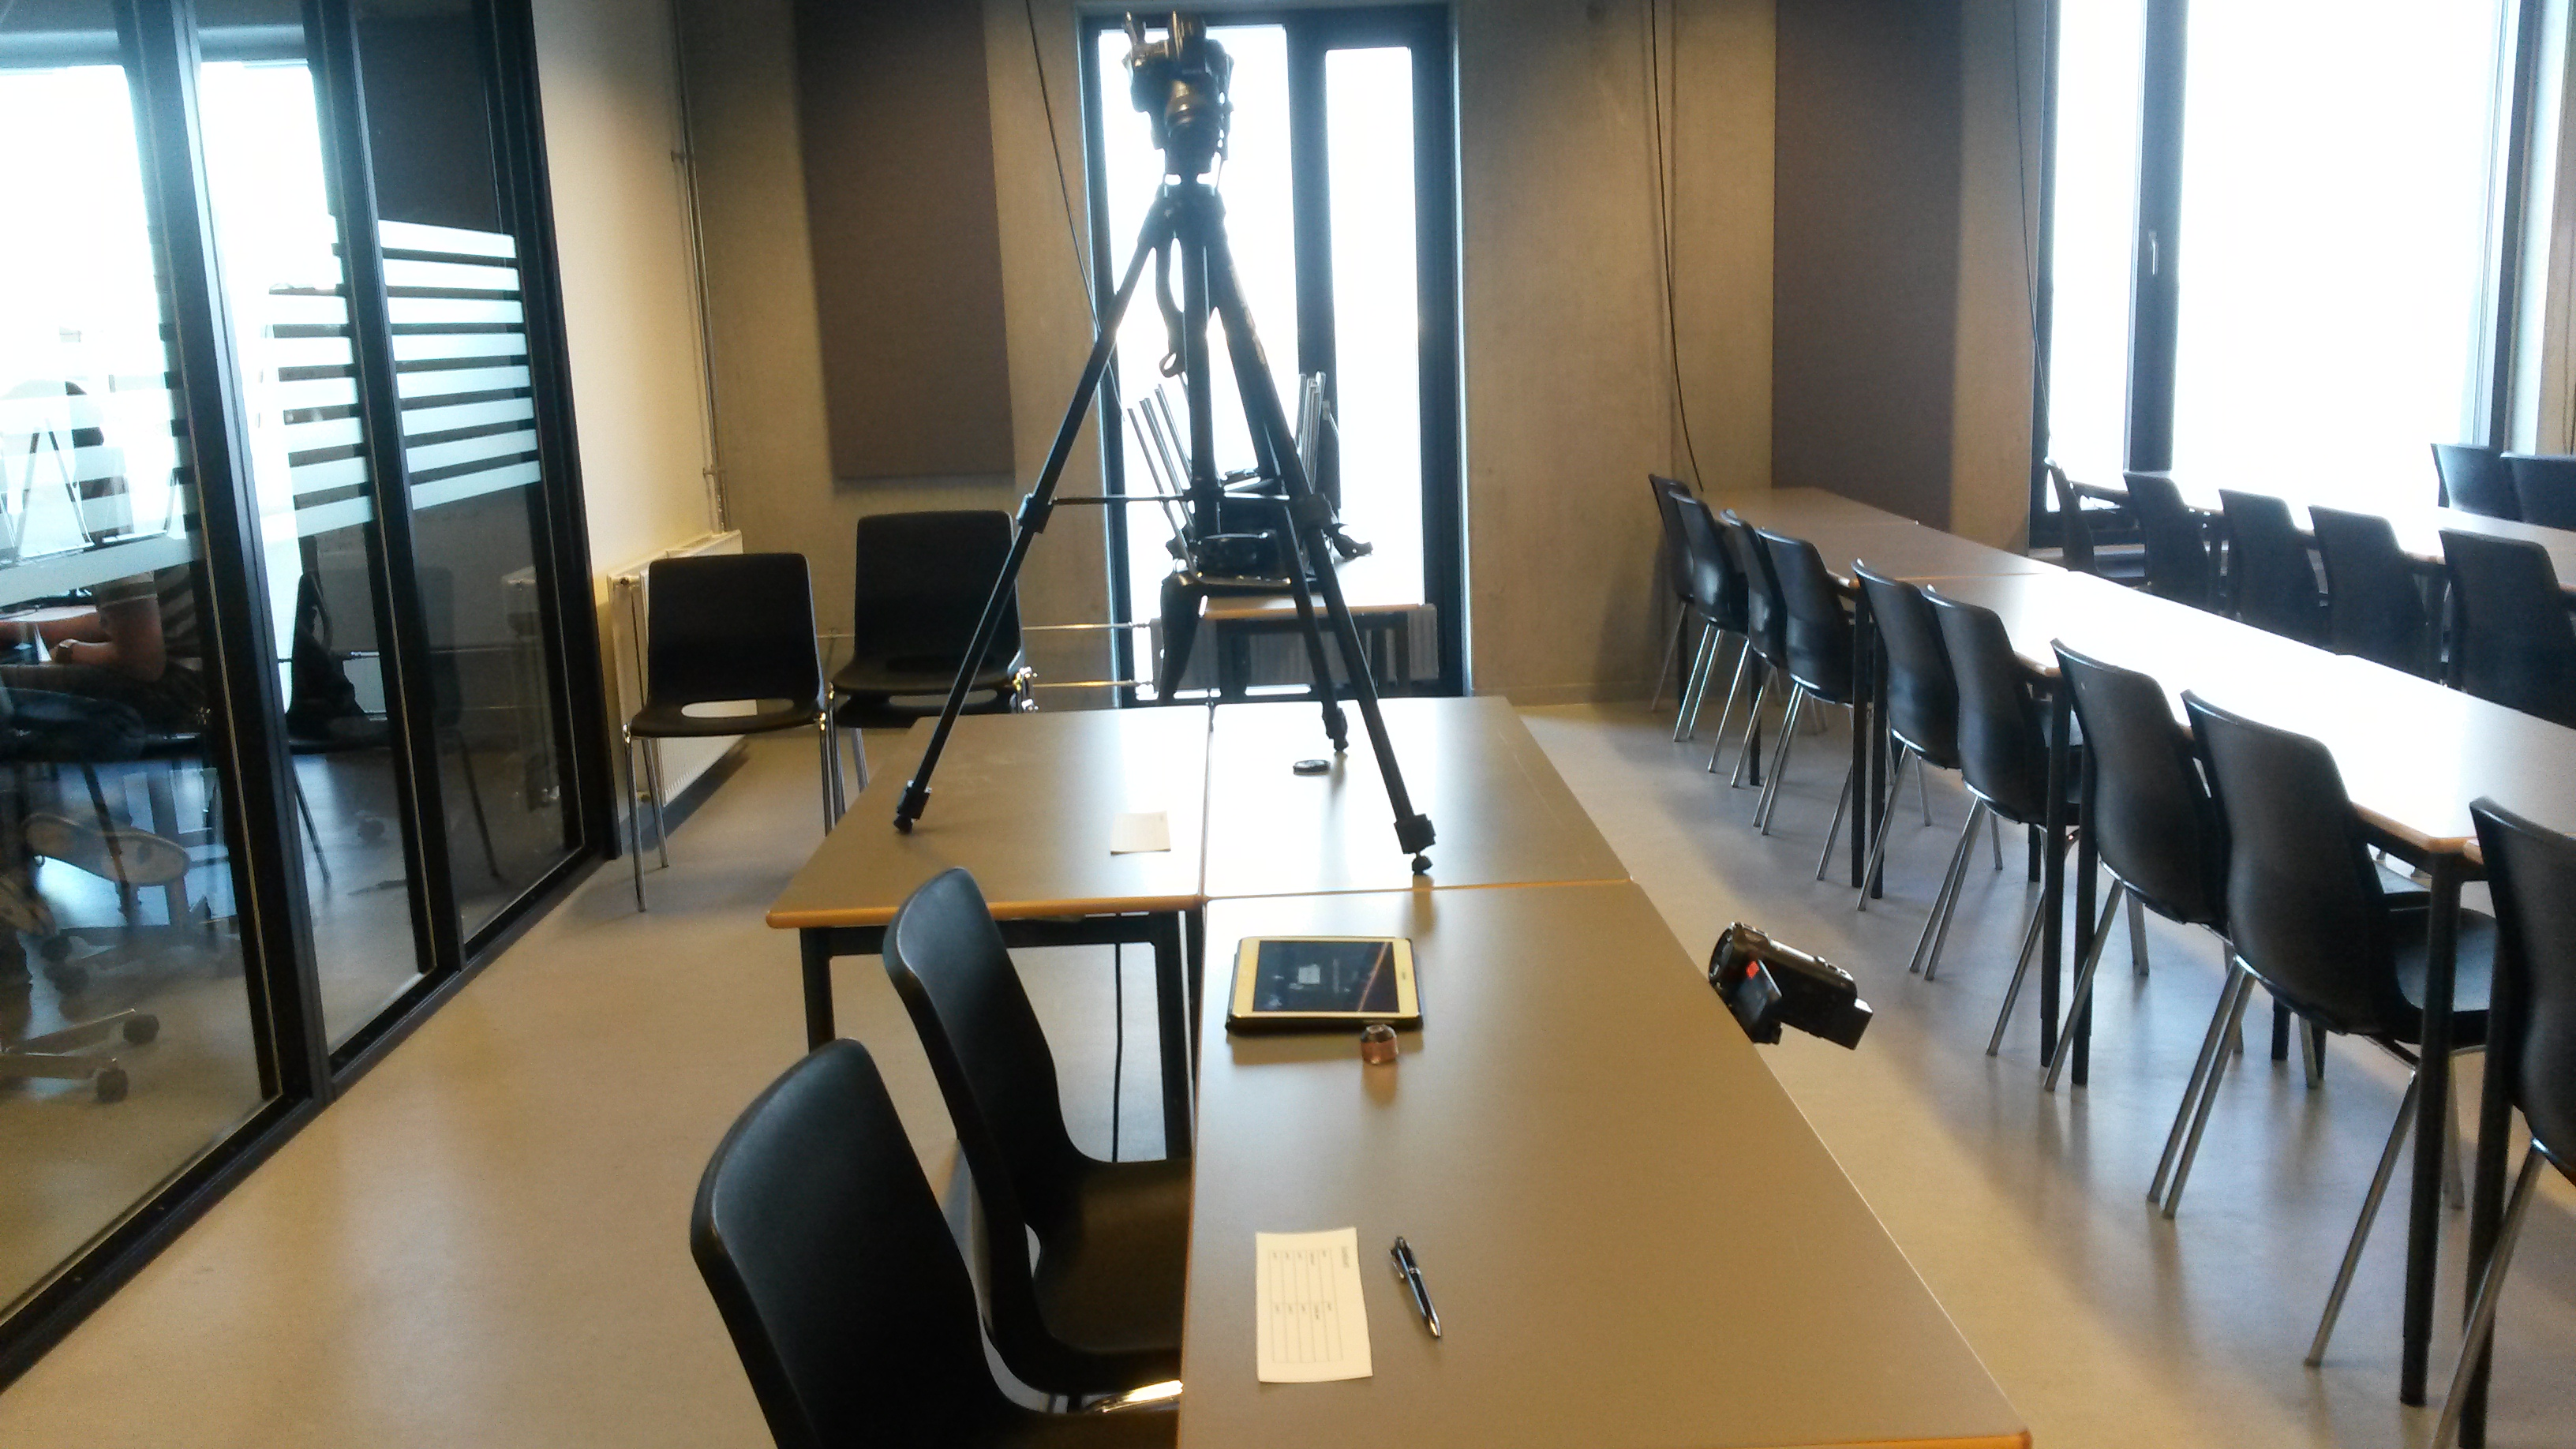
\includegraphics[width=0.75\textwidth]{img/setup}
\caption{Camera setup for the tests.}
\end{figure}\label{fig: cam_set}

\begin{table}
\begin{tabular}{|c|c|c|c|c|}
\hline 
Session 1 & Session 2 & Session 3 & Session 4 & Session 5 \\ 
\hline 
Male/Male & Male/Female & Female/Male & Female/Female & Male/Female \\ 
\hline 
\end{tabular} 
\caption{The table illustrates the combination of gender in the test. The second entry for all session (labeled as B) was the second participant, who experienced the rigged level.}
\end{table}\label{tab: pairs}
